\chapter{Bilangan Kuantum dan Konfigurasi Elektron}\label{ch:b1:quantum-numbers}

Isilah sebuah tabung kaca dengan hidrogen bertekanan rendah, alirkan
lucutan listrik melaluinya, lalu amati pendar merah mudanya melalui
sebuah prisma. Cahayanya tidak terurai menjadi pelangi, tetapi terpecah
menjadi empat garis tajam --- satu merah, satu hijau kebiruan, dua ungu
--- tanpa apa pun di antaranya. Padatan yang panas memancar pada semua
panjang gelombang; atom hidrogen hanya memancarkan segelintir. Penjelasannya,
yang ditemukan antara tahun 1913 dan 1926, ialah bahwa energi elektron di
dalam atom tidak dapat mengambil sembarang nilai: energi itu
\emph{terkuantisasi}. Bab ini menyatakan aturan-aturan kuantisasi itu
sebagaimana dipakai ahli kimia --- empat bilangan kuantum, tiga aturan
pengisian --- dan mengubahnya menjadi \omterm{def:b1:quantum-numbers:configuration}{konfigurasi elektron} setiap atom
dan ion, kunci tabel periodik pada bab berikutnya.

\begin{recall}
Buku 1 (kelas 10) menempatkan elektron dua puluh unsur pertama dalam
kulit dan \omterm{def:b1:quantum-numbers:orbital}{subkulit}, 1s, 2s, 2p, 3s, 3p, dan menyebut elektron kulit
terluar sebagai \omterm{def:b1:quantum-numbers:configuration}{elektron valensinya}. Dari fisika kita memakai, sebagai
hal yang sudah diketahui, bahwa cahaya dengan panjang gelombang $\lambda$
tersusun atas foton berenergi $E = h\nu = hc/\lambda$, dengan $h$ tetapan
Planck dan $c$ kelajuan cahaya.
\end{recall}

\begin{omfigure}
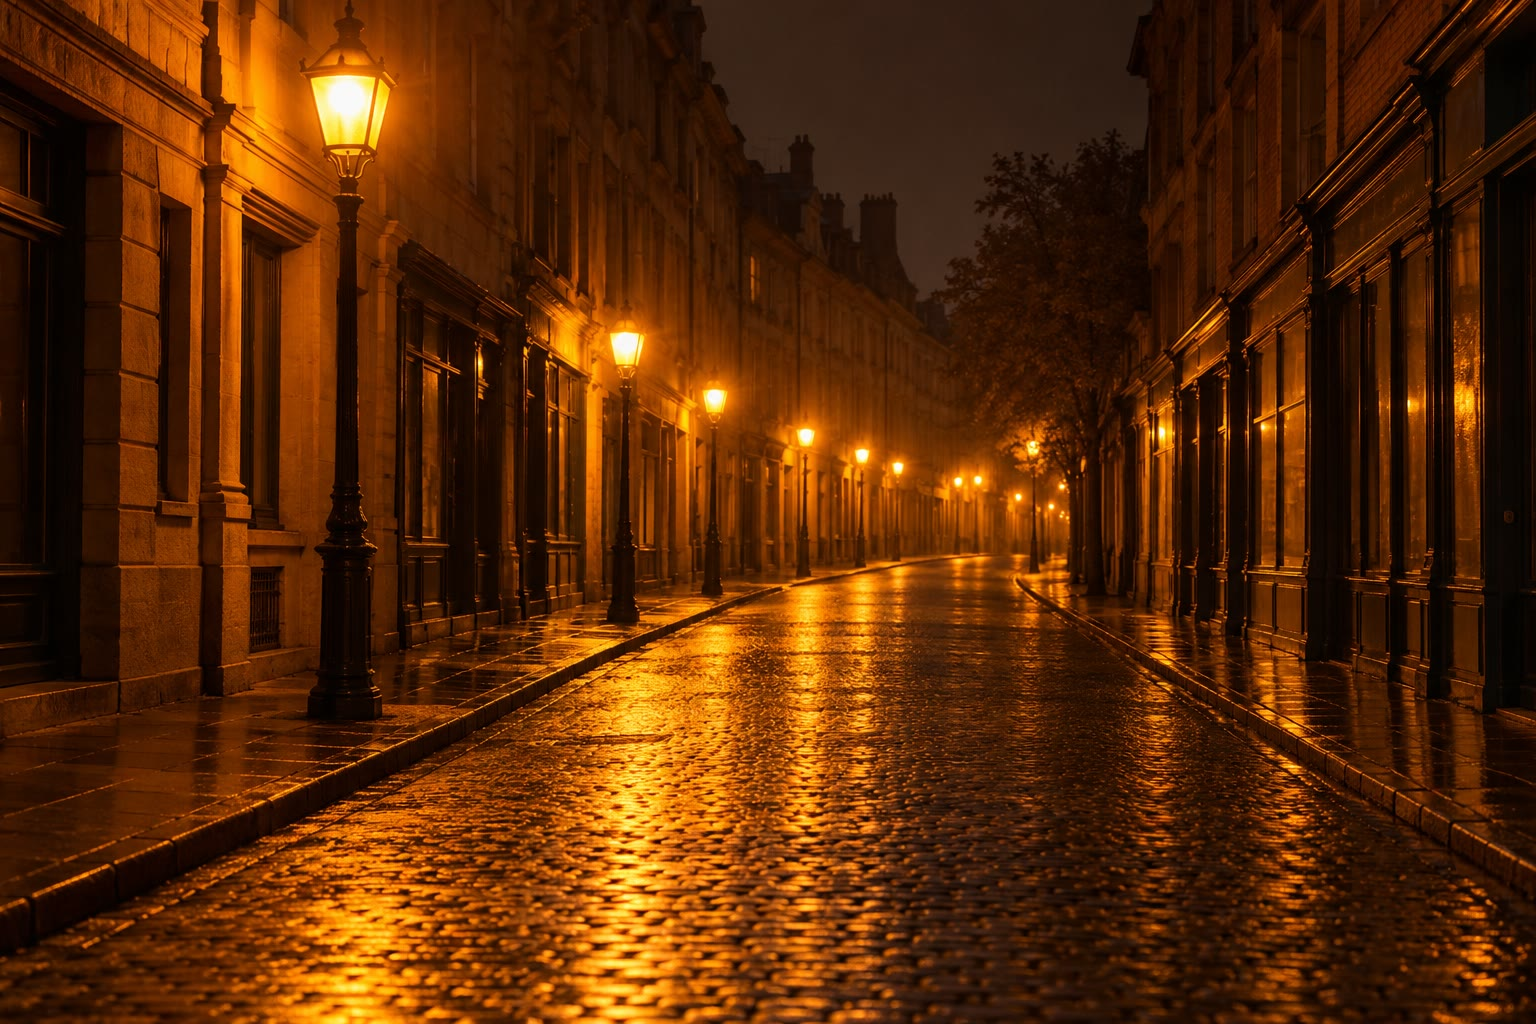
\includegraphics[width=0.62\linewidth]{images/book2/ai/b1-01-street-lamps.jpg}

{\small Lampu jalan natrium bertekanan rendah. Cahayanya hampir berupa
satu garis jingga-kuning: seperti hidrogen, atom natrium yang tereksitasi
hanya memancarkan foton dengan beberapa energi yang tepat.}
\end{omfigure}

\section{Energi terkuantisasi: spektrum hidrogen}

\begin{definition}[Tingkat energi, keadaan dasar, keadaan tereksitasi]\label{def:b1:quantum-numbers:energy-level}
Energi elektron yang terikat di dalam atom hanya dapat mengambil
nilai-nilai tertentu, yaitu \emph{tingkat energi}\index{tingkat energi}
atom tersebut. Nol energi diambil ketika elektron diam di tempat yang
jauhnya tak berhingga dari inti (atom terionisasi), sehingga setiap
tingkat elektron terikat bernilai negatif. Tingkat terendah adalah
\emph{keadaan dasar}\index{keadaan dasar}; setiap tingkat lainnya adalah
\emph{keadaan tereksitasi}\index{keadaan tereksitasi}.
\end{definition}

Atom berpindah dari tingkat berenergi $E_{\text{tinggi}}$ ke tingkat yang
lebih rendah $E_{\text{rendah}}$ dengan memancarkan satu foton, dan dari
tingkat yang lebih rendah ke yang lebih tinggi dengan menyerap satu foton,
yang energinya
\[
  h\nu = \frac{hc}{\lambda} = E_{\text{tinggi}} - E_{\text{rendah}} .
\]
Jadi, spektrum garis adalah gambaran selisih antartingkat energi.

\begin{theorem}[Tingkat energi atom hidrogen]\label{thm:b1:quantum-numbers:levels}
\omterm{def:b1:quantum-numbers:energy-level}{Tingkat energi} atom hidrogen adalah
\[
  E_n = -\frac{E_R}{n^2}, \qquad n = 1, 2, 3, \dots,
  \qquad E_R = \qty{13.6}{eV},
\]
dengan $E_R$ energi Rydberg (dikoreksi terhadap gerak inti). \omterm{def:b1:quantum-numbers:energy-level}{Keadaan
dasarnya} adalah $E_1 = \qty{-13.6}{eV}$ dan energi ionisasi atom itu
adalah $E_R$.
% ledger: const:RyhcEV, ie:H (13.598 eV; levels computed in
% figdata/bachelor-1/hydrogen-levels.py)
\end{theorem}
\admitted

\begin{remark}[Asal rumus ini]\label{rem:b1:quantum-numbers:schrodinger}
Rumus ini diperoleh dengan menyelesaikan persamaan Schrödinger untuk
elektron di dalam medan proton; penyelesaiannya, serta bentuk fungsi
gelombang yang dihasilkannya, diturunkan dalam jilid Tahun 2. Niels Bohr
telah memperoleh tingkat-tingkat yang sama pada tahun 1913 dari model
orbit lingkaran yang lebih sederhana, yang kini telah ditinggalkan.
\end{remark}

\begin{proposition}[Rumus Rydberg]\label{prop:b1:quantum-numbers:rydberg}
Garis-garis yang dipancarkan hidrogen mempunyai panjang gelombang
\[
  \frac{1}{\lambda} = R_H\left(\frac{1}{n_1^2} - \frac{1}{n_2^2}\right),
  \qquad n_2 > n_1 \ge 1, \qquad R_H = \frac{E_R}{hc},
\]
untuk transisi dari tingkat $n_2$ turun ke tingkat $n_1$. Garis-garis
yang berakhir pada tingkat $n_1$ yang sama membentuk sebuah
\emph{deret}: Lyman untuk $n_1 = 1$ (ultraungu), Balmer untuk $n_1 = 2$
(tampak), Paschen untuk $n_1 = 3$ (inframerah).
\end{proposition}

\begin{proof}
Foton membawa energi yang dilepaskan atom:
$hc/\lambda = E_{n_2} - E_{n_1} = -E_R/n_2^2 + E_R/n_1^2
= E_R\,(1/n_1^2 - 1/n_2^2)$. Dengan membaginya dengan $hc$, diperoleh rumus tersebut.
\end{proof}

\begin{example}[Garis merah hidrogen]\label{ex:b1:quantum-numbers:halpha}
Untuk transisi $3 \to 2$: $\Delta E = 13.6\,(1/4 - 1/9) =
\qty{1.89}{eV}$. Dengan $hc = \qty{1240}{eV.nm}$ (dari nilai $h$,
$c$, dan $e$), $\lambda = 1240/1.89 = \qty{656}{nm}$: garis merah.
Garis-garis Balmer lainnya, $4 \to 2$, $5 \to 2$, $6 \to 2$, jatuh pada
486, 434, dan \qty{410}{nm}; garis berikutnya, $7 \to 2$ pada
\qty{397}{nm}, sudah berada di daerah ultraungu. Panjang gelombang
terukur, 656.3, 486.1, 434.0, dan \qty{410.2}{nm}, cocok dengan
ketelitian lebih baik daripada satu per dua ribu; selisih kecil yang
tersisa berasal dari pengukuran di udara, bukan di vakum.
% ledger: asd:Halpha, asd:Hbeta, asd:Hgamma, asd:Hdelta (computed values
% in figdata/out/bachelor-1-hydrogen-levels-balmer.dat)
\end{example}

\begin{omfigure}
\begin{tikzpicture}
\begin{axis}[
  width=0.62\linewidth, height=7.2cm,
  xmin=0, xmax=10, ymin=-14.5, ymax=0.6,
  axis x line=none, axis y line=left,
  ylabel={energi (eV)}, ytick={-14,-12,-10,-8,-6,-4,-2,0},
  tick label style={font=\small}, label style={font=\small},
  clip=false]
\pgfplotsinvokeforeach{-13.598,-3.400,-1.511,-0.850,-0.544}{
  \draw[black!70, line width=0.7pt] (axis cs:0.3,#1) -- (axis cs:9.6,#1);}
\draw[black!40, dashed] (axis cs:0.3,0) -- (axis cs:9.6,0);
\node[font=\small, anchor=west] at (axis cs:9.7,-13.598) {$n = 1$};
\node[font=\small, anchor=west] at (axis cs:9.7,-3.400) {$n = 2$};
\node[font=\small, anchor=west] at (axis cs:9.7,-1.511) {$n = 3$};
\node[font=\small, anchor=south west] at (axis cs:9.7,0.05) {$n \to \infty$};
% Lyman
\draw[-{Stealth}, violet!70!black, thick] (axis cs:1.0,-3.400) -- (axis cs:1.0,-13.598);
\draw[-{Stealth}, violet!70!black, thick] (axis cs:1.6,-1.511) -- (axis cs:1.6,-13.598);
\draw[-{Stealth}, violet!70!black, thick] (axis cs:2.2,-0.850) -- (axis cs:2.2,-13.598);
\node[font=\small, violet!70!black, anchor=west] at (axis cs:2.4,-9) {Lyman};
% Balmer
\draw[-{Stealth}, red!80!black, thick] (axis cs:4.4,-1.511) -- (axis cs:4.4,-3.400);
\draw[-{Stealth}, teal!80!black, thick] (axis cs:5.0,-0.850) -- (axis cs:5.0,-3.400);
\draw[-{Stealth}, blue!80!black, thick] (axis cs:5.6,-0.544) -- (axis cs:5.6,-3.400);
\node[font=\small, anchor=north] at (axis cs:5.0,-3.6) {Balmer};
% Paschen
\draw[-{Stealth}, black!60, thick] (axis cs:7.8,-0.850) -- (axis cs:7.8,-1.511);
\draw[-{Stealth}, black!60, thick] (axis cs:8.4,-0.544) -- (axis cs:8.4,-1.511);
\node[font=\small, anchor=north] at (axis cs:8.1,-1.7) {Paschen};
\end{axis}
\end{tikzpicture}

{\small Tingkat-tingkat energi hidrogen, $E_n = -\qty{13.6}{eV}/n^2$,
digambar dengan skala sebenarnya (dihitung dari tetapan Rydberg);
tingkat $n = 4,
5, \dots$ berdesakan di bawah nol. Setiap panah adalah
satu foton yang dipancarkan; panah-panah yang berakhir pada tingkat yang
sama membentuk satu deret.}
\end{omfigure}

\begin{omfigure}
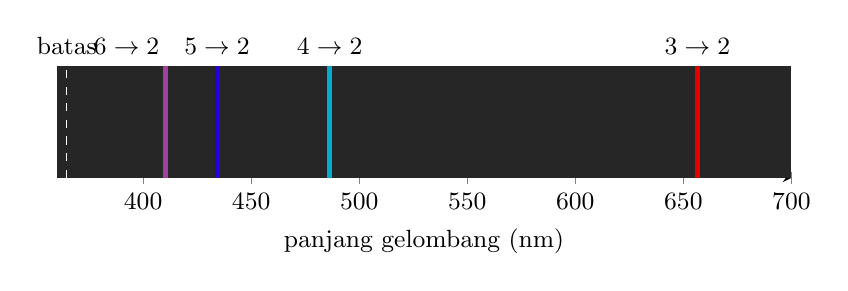
\begin{tikzpicture}
\begin{axis}[
  width=0.9\linewidth, height=3.0cm,
  xmin=360, xmax=700, ymin=0, ymax=1,
  axis x line=bottom, axis y line=none,
  xlabel={panjang gelombang (nm)}, xtick={400,450,500,550,600,650,700},
  tick label style={font=\small}, label style={font=\small},
  clip=false]
\fill[black!85] (axis cs:360,0) rectangle (axis cs:700,1);
% line positions: figdata/out/bachelor-1-hydrogen-levels-balmer.dat
\draw[line width=1.6pt, red!90!black] (axis cs:656.5,0) -- (axis cs:656.5,1);
\draw[line width=1.6pt, cyan!80!green] (axis cs:486.3,0) -- (axis cs:486.3,1);
\draw[line width=1.6pt, blue!70!violet] (axis cs:434.2,0) -- (axis cs:434.2,1);
\draw[line width=1.6pt, violet!75] (axis cs:410.3,0) -- (axis cs:410.3,1);
\draw[white, dashed] (axis cs:364.7,0) -- (axis cs:364.7,1);
\node[font=\small, anchor=south] at (axis cs:364.7,1.02) {batas};
\node[font=\small, anchor=south] at (axis cs:656.5,1.02) {$3\to2$};
\node[font=\small, anchor=south] at (axis cs:486.3,1.02) {$4\to2$};
\node[font=\small, anchor=south] at (axis cs:434.2,1.02) {$5\to2$};
\node[font=\small, anchor=south east] at (axis cs:412,1.02) {$6\to2$};
\end{axis}
\end{tikzpicture}

{\small Garis-garis Balmer yang dihitung dari rumus Rydberg (panjang
gelombang di vakum), pada pita cahaya tampak. Garis-garis berikutnya
berdesakan menuju batas deret pada \qty{364.7}{nm}, di daerah ultraungu.}
\end{omfigure}

\begin{history}[Atom Bohr, 1913]
Pada tahun 1913 Niels Bohr, fisikawan Denmark berusia 28 tahun yang
bekerja di Manchester, mengusulkan bahwa elektron hidrogen hanya dapat
mengelilingi inti pada orbit-orbit tertentu, dan bahwa cahaya dipancarkan
ketika elektron itu melompat dari satu orbit ke orbit yang lebih rendah.
Modelnya menghasilkan garis-garis Balmer dengan tepat, juga nilai tetapan
Rydberg dari $h$, $e$, dan massa elektron. Orbit-orbit itu tidak bertahan
menghadapi mekanika kuantum tahun 1925--1926, tetapi tingkat-tingkat yang
terkuantisasi bertahan. Bohr menerima Hadiah Nobel Fisika pada tahun 1922.
\end{history}

\begin{omfigure}
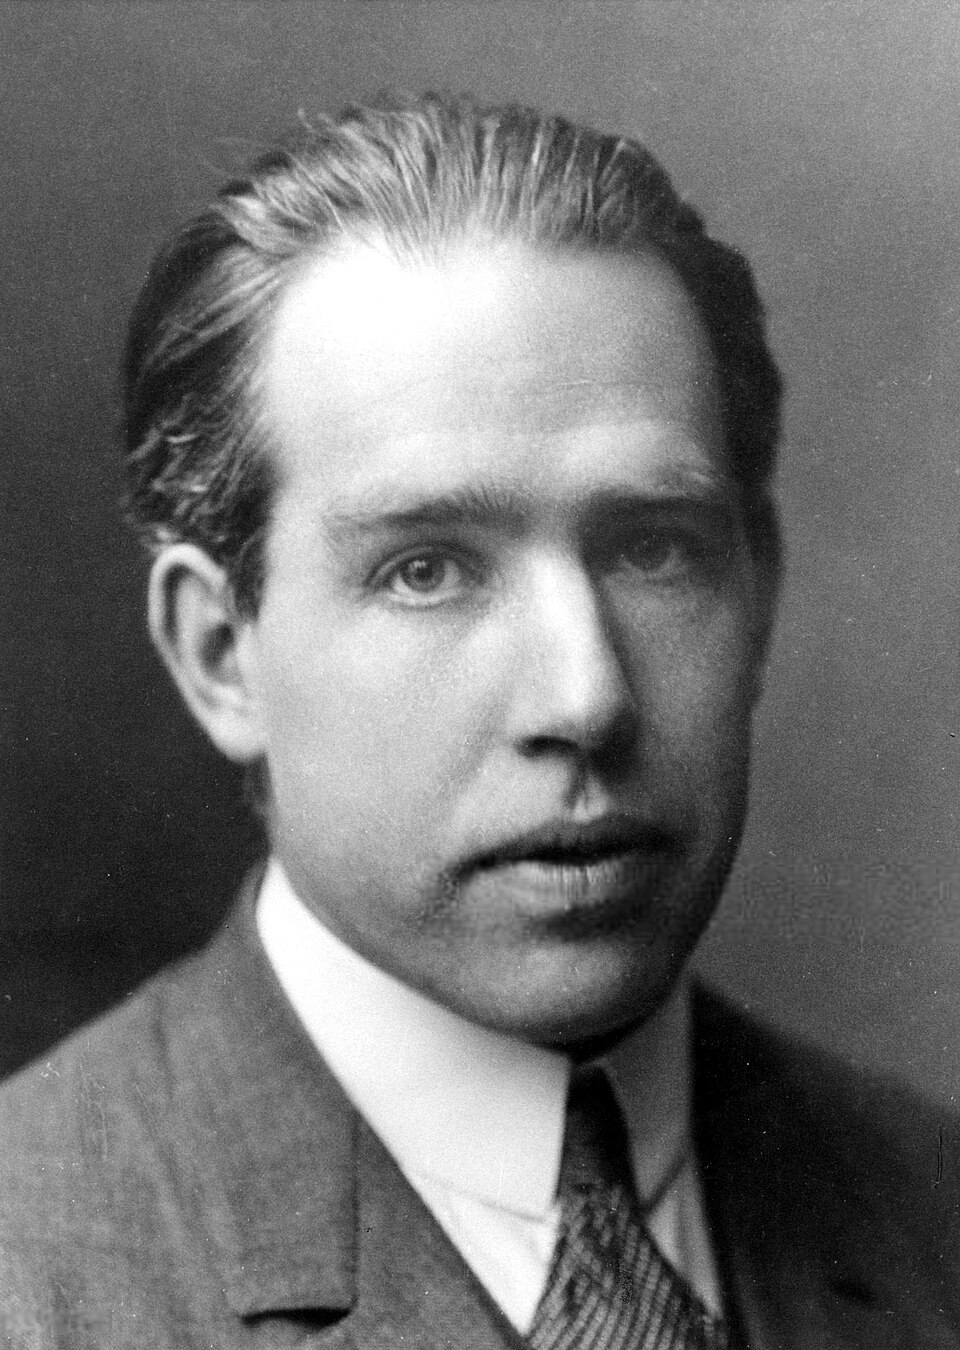
\includegraphics[width=0.26\linewidth]{images/book2/bohr.jpg}

{\small Niels Bohr (1885--1962), sekitar tahun 1922.}
\end{omfigure}

\section{Empat bilangan kuantum}

Di dalam atom berelektron banyak, energi tidak lagi diberikan oleh satu
rumus, tetapi setiap elektron tetap dicirikan oleh sekumpulan kecil
bilangan bulat, yaitu bilangan-bilangan kuantumnya.

\begin{definition}[Bilangan kuantum]\label{def:b1:quantum-numbers:quantum-number}
Keadaan sebuah elektron di dalam atom ditandai oleh empat bilangan:
\begin{itemize}
  \item \emph{bilangan kuantum utama}\index{bilangan kuantum utama}
        $n = 1, 2, 3, \dots$, yang terutama menentukan energi dan ukuran;
  \item \emph{bilangan kuantum azimut}\index{bilangan kuantum azimut}
        (atau bilangan kuantum sekunder) $l = 0, 1, \dots, n-1$, yang
        menentukan bentuk; $l = 0, 1, 2, 3$ ditulis s, p, d, f;
  \item \emph{bilangan kuantum magnetik}\index{bilangan kuantum magnetik}
        $m_l = -l, -l+1, \dots, l$, yang menentukan orientasi ($2l + 1$
        nilai);
  \item \emph{bilangan kuantum spin}\index{bilangan kuantum spin}
        $m_s = +\tfrac12$ atau $-\tfrac12$, sifat intrinsik elektron,
        yang digambar sebagai panah ke atas atau ke bawah.
\end{itemize}
\end{definition}

\begin{definition}[Orbital atom, kulit, subkulit]\label{def:b1:quantum-numbers:orbital}
\emph{Orbital atom}\index{orbital atom} adalah keadaan satu elektron
yang ditandai oleh tiga bilangan $(n, l, m_l)$; orbital digambar sebagai
satu kotak, \omorbs{}. Orbital-orbital dengan $n$ yang sama membentuk
sebuah \emph{kulit elektron}\index{kulit elektron}; orbital-orbital
dengan $n$ dan $l$ yang sama membentuk sebuah
\emph{subkulit}\index{subkulit}, yang dinamai menurut $n$ dan huruf $l$:
2p adalah subkulit $n = 2$, $l = 1$, yang terdiri atas tiga orbital
($m_l = -1, 0, 1$).
\end{definition}

\begin{remark}[Bentuk orbital]\label{rem:b1:quantum-numbers:shapes}
Orbital s berbentuk bola; orbital p mempunyai dua cuping di sepanjang
sebuah sumbu, dan ketiga orbital 2p mengarah sepanjang $x$, $y$, dan $z$.
Deskripsi matematis bentuk-bentuk ini --- fungsi gelombang, bagian radial
dan bagian angularnya, simpul-simpulnya --- termasuk jilid Tahun 2. Dalam
buku ini orbital adalah sebuah kotak yang memuat paling banyak dua
elektron.
\end{remark}

\begin{proposition}[Kapasitas subkulit dan kulit]\label{prop:b1:quantum-numbers:capacity}
\omterm{def:b1:quantum-numbers:orbital}{Subkulit} dengan bilangan azimut $l$ memuat $2l + 1$ orbital dan dapat
menampung $2(2l + 1)$ elektron: 2 pada s, 6 pada p, 10 pada d, 14 pada f.
Kulit $n$ memuat $n^2$ orbital dan dapat menampung $2n^2$ elektron.
\end{proposition}

\begin{proof}
Untuk $l$ tertentu, $m_l$ mengambil $2l + 1$ nilai dari $-l$ sampai $l$,
dan setiap orbital memuat dua elektron dengan spin berlawanan
(\cref{prop:b1:quantum-numbers:pauli} di bawah). Untuk $n$ tertentu, $l$
berjalan dari $0$ sampai $n - 1$, sehingga banyaknya orbital adalah
\[
  \sum_{l=0}^{n-1} (2l+1) = 2\,\frac{(n-1)n}{2} + n = n^2 ,
\]
dan banyaknya elektron adalah $2n^2$: 2, 8, 18, 32 untuk $n = 1$ sampai 4.
\end{proof}

\begin{example}[Kulit ketiga]\label{ex:b1:quantum-numbers:third}
Untuk $n = 3$: $l = 0$ (3s, satu orbital), $l = 1$ (3p, tiga orbital),
$l = 2$ (3d, lima orbital, $m_l = -2, \dots, 2$): sembilan orbital dan
paling banyak 18 elektron. Sebuah elektron pada 3d mempunyai, misalnya,
bilangan kuantum $(3, 2, -1, +\tfrac12)$.
\end{example}

\section{Menyusun konfigurasi}

\begin{definition}[Konfigurasi elektron]\label{def:b1:quantum-numbers:configuration}
\emph{Konfigurasi elektron}\index{konfigurasi elektron} sebuah atom atau
ion adalah daftar \omterm{def:b1:quantum-numbers:orbital}{subkulit} yang terisi beserta banyaknya elektron pada
masing-masing, yang ditulis sebagai pangkat: $1\text{s}^2 2\text{s}^2
2\text{p}^4$ untuk oksigen. Elektron-elektron dengan $n$ tertinggi,
bersama elektron \omterm{def:b1:quantum-numbers:orbital}{subkulit} d atau f yang belum terisi penuh, adalah
\emph{elektron valensi}\index{elektron valensi}; elektron lainnya adalah
\emph{elektron teras}\index{elektron teras}. Konfigurasi disingkat dengan
menuliskan konfigurasi gas mulia sebelumnya di dalam kurung siku:
oksigen adalah $[\ce{He}]\,2\text{s}^2 2\text{p}^4$.
\end{definition}

Tiga aturan menghasilkan konfigurasi \omterm{def:b1:quantum-numbers:energy-level}{keadaan dasar}.

\begin{proposition}[Asas larangan Pauli]\label{prop:b1:quantum-numbers:pauli}
Dua elektron dalam atom yang sama tidak pernah mempunyai keempat bilangan
kuantum yang sama. Akibatnya, satu orbital memuat paling banyak dua
elektron, dan keduanya berspin berlawanan: \omorbs{ud}.
\end{proposition}
\admitted

\begin{proposition}[Aturan Klechkowski]\label{prop:b1:quantum-numbers:klechkowski}
Pada \omterm{def:b1:quantum-numbers:energy-level}{keadaan dasar} atom netral, \omterm{def:b1:quantum-numbers:orbital}{subkulit-subkulit} diisi menurut urutan
$n + l$ yang membesar, dan untuk $n + l$ yang sama menurut urutan $n$ yang
membesar:
\[
  1\text{s},\ 2\text{s},\ 2\text{p},\ 3\text{s},\ 3\text{p},\ 4\text{s},\
  3\text{d},\ 4\text{p},\ 5\text{s},\ 4\text{d},\ 5\text{p},\ 6\text{s},\
  4\text{f},\ 5\text{d},\ 6\text{p},\ 7\text{s},\ 5\text{f},\ 6\text{d},\
  7\text{p}.
\]
\end{proposition}
\admitted

\begin{remark}[Aturan empiris]\label{rem:b1:quantum-numbers:klech-empirical}
Aturan Klechkowski (disebut juga aturan Madelung) adalah ringkasan
konfigurasi yang teramati, bukan hukum: aturan itu memerikan urutan
pengisian \omterm{def:b1:quantum-numbers:orbital}{subkulit} seiring bertambahnya muatan inti. Di dalam atom
berelektron banyak, elektron-elektron saling tolak, sehingga energi
sebuah \omterm{def:b1:quantum-numbers:orbital}{subkulit} bergantung pada $l$ dan juga pada $n$: elektron 4s, yang
menghabiskan sebagian waktunya di dekat inti, akhirnya berada di bawah
3d pada kalium dan kalsium.
\end{remark}

\begin{omfigure}
\begin{tikzpicture}[font=\small, x=1.25cm, y=0.72cm]
  \foreach \n in {1,...,7} {
    \foreach \l/\s in {0/s,1/p,2/d,3/f} {
      \pgfmathtruncatemacro\ok{(\l<\n) && (\n+\l<=8)}
      \ifnum\ok=1
        \node[draw=black!50, rounded corners=2pt, minimum width=0.85cm,
          minimum height=0.5cm, fill=white] (s\n\l) at (\l,-\n) {\n\s};
      \fi
    }
  }
  \begin{scope}[on background layer]
  \foreach \la/\na/\lb/\nb in {0/1/0/1, 0/2/0/2, 1/2/0/3, 1/3/0/4, 2/3/0/5,
      2/4/0/6, 3/4/0/7, 3/5/1/7} {
    \draw[-{Stealth}, omDef, thick, opacity=0.8]
      ($(\la,-\na)+(0.5,0.42)$) -- ($(\lb,-\nb)+(-0.5,-0.42)$);
  }
  \end{scope}
  \node[anchor=west, align=left, font=\small] at (4.0,-2.5) {ikuti setiap panah,\\lalu panah berikutnya\\di sebelah kanannya};
\end{tikzpicture}

{\small Diagram Klechkowski. \omterm{def:b1:quantum-numbers:orbital}{Subkulit-subkulit} dengan $n + l$ yang sama
terletak pada satu diagonal; mengikuti diagonal-diagonal itu secara
berurutan menghasilkan urutan pengisian 1s, 2s, 2p, 3s, 3p, 4s, 3d, 4p,
5s, \dots}
\end{omfigure}

\begin{proposition}[Aturan Hund]\label{prop:b1:quantum-numbers:hund}
Jika elektron-elektron sebuah \omterm{def:b1:quantum-numbers:orbital}{subkulit} dapat ditempatkan pada beberapa
orbital yang berenergi sama, \omterm{def:b1:quantum-numbers:energy-level}{keadaan dasarnya} mempunyai banyak spin
\emph{sejajar} sebesar mungkin: elektron-elektron menempati orbital yang
terpisah, dengan spin ke atas, sebelum satu orbital pun terisi ganda.
\end{proposition}
\admitted

\begin{definition}[Elektron tak berpasangan]\label{def:b1:quantum-numbers:unpaired}
\emph{Elektron tak berpasangan}\index{elektron tak berpasangan} adalah
elektron yang sendirian di dalam orbitalnya. Spesies yang mempunyai
elektron tak berpasangan ditarik oleh magnet (spesies itu bersifat
paramagnetik, sifat yang dipelajari dalam fisika).
\end{definition}

\begin{method}[Menuliskan konfigurasi keadaan dasar]\label{met:b1:quantum-numbers:configuration}
Untuk menuliskan konfigurasi atom bernomor atom $Z$:
\begin{enumerate}
  \item tempatkan $Z$ elektron pada \omterm{def:b1:quantum-numbers:orbital}{subkulit-subkulit} menurut urutan
        Klechkowski, dengan mengisi penuh setiap \omterm{def:b1:quantum-numbers:orbital}{subkulit} (2, 6, 10, 14)
        sebelum \omterm{def:b1:quantum-numbers:orbital}{subkulit} berikutnya;
  \item tuliskan hasilnya menurut urutan $n$ yang membesar
        (mengelompokkan 3d dengan $n = 3$), lalu singkat dengan teras gas
        mulia sebelumnya;
  \item untuk \omterm{def:b1:quantum-numbers:orbital}{subkulit} terakhir yang belum terisi penuh, gambarlah
        kotak-kotaknya dan terapkan aturan Hund untuk menghitung \omterm{def:b1:quantum-numbers:unpaired}{elektron
        tak berpasangan}.
\end{enumerate}
\end{method}

\begin{example}[Karbon, nitrogen, oksigen, besi]\label{ex:b1:quantum-numbers:examples}
Metode ini menghasilkan, untuk empat atom:
\begin{center}
\begin{tabular}{lllc}
\hline
atom & konfigurasi & \omterm{def:b1:quantum-numbers:orbital}{subkulit} terakhir & tak berpasangan \\
\hline
\ce{C} ($Z = 6$) & $[\ce{He}]\,2\text{s}^2 2\text{p}^2$ & 2p: \omorbs{u,u,} & 2 \\
\ce{N} ($Z = 7$) & $[\ce{He}]\,2\text{s}^2 2\text{p}^3$ & 2p: \omorbs{u,u,u} & 3 \\
\ce{O} ($Z = 8$) & $[\ce{He}]\,2\text{s}^2 2\text{p}^4$ & 2p: \omorbs{ud,u,u} & 2 \\
\ce{Fe} ($Z = 26$) & $[\ce{Ar}]\,3\text{d}^6 4\text{s}^2$ & 3d: \omorbs{ud,u,u,u,u} & 4 \\
\hline
\end{tabular}
\end{center}
Pada besi, urutan Klechkowski mengisi 4s ($Z = 19, 20$) sebelum 3d
($Z = 21$ sampai 30); konfigurasinya ditulis dengan 3d lebih dahulu.
% ledger: gs:Fe
\end{example}

\begin{omfigure}
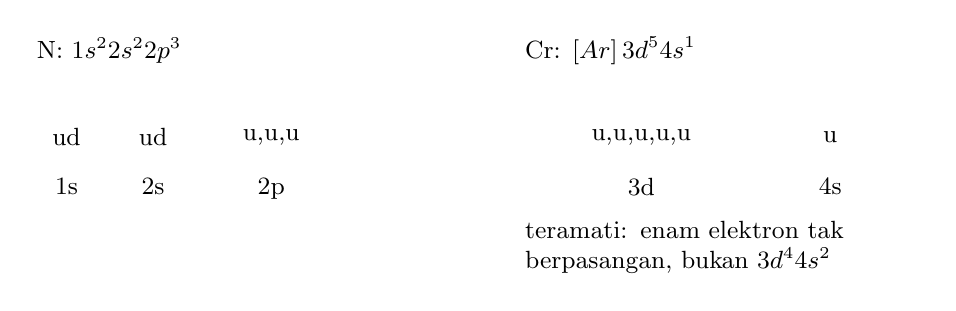
\begin{tikzpicture}[font=\small]
  \begin{scope}
    \node[anchor=west] at (0,2.4) {\ce{N}: $1\text{s}^2 2\text{s}^2 2\text{p}^3$};
    \node at (0.5,1.3) {\omorbs{ud}}; \node[below] at (0.5,0.9) {1s};
    \node at (1.6,1.3) {\omorbs{ud}}; \node[below] at (1.6,0.9) {2s};
    \node at (3.1,1.3) {\omorbs{u,u,u}}; \node[below] at (3.1,0.9) {2p};
  \end{scope}
  \begin{scope}[xshift=6.2cm]
    \node[anchor=west] at (0,2.4) {\ce{Cr}: $[\ce{Ar}]\,3\text{d}^5 4\text{s}^1$};
    \node at (1.6,1.3) {\omorbs{u,u,u,u,u}}; \node[below] at (1.6,0.9) {3d};
    \node at (4.0,1.3) {\omorbs{u}}; \node[below] at (4.0,0.9) {4s};
    \node[anchor=west, text width=5.0cm] at (0,-0.1) {teramati: enam elektron tak berpasangan, bukan $3\text{d}^4 4\text{s}^2$};
  \end{scope}
\end{tikzpicture}

{\small Kotak kuantum. Setiap kotak adalah satu orbital; sebuah panah
adalah satu elektron beserta spinnya. Nitrogen mengikuti aturan Hund;
kromium adalah salah satu pengecualian pada
\cref{prop:b1:quantum-numbers:exceptions}.}
\end{omfigure}

\section{Ion, pengecualian, dan bentuk tabel periodik}

\begin{proposition}[Konfigurasi ion]\label{prop:b1:quantum-numbers:ions}
Anion monoatomik mempunyai konfigurasi atomnya dengan elektron tambahan
yang ditempatkan pada posisi berikutnya dalam urutan Klechkowski; kation
unsur golongan utama melepaskan elektron dengan $n$ tertinggi. Kation
logam transisi melepaskan elektron $n$s-nya \emph{sebelum} elektron
$(n-1)$d-nya: \ce{Fe^{2+}} adalah $[\ce{Ar}]\,3\text{d}^6$ dan
\ce{Fe^{3+}} adalah $[\ce{Ar}]\,3\text{d}^5$, bukan $[\ce{Ar}]\,3\text{d}^4
4\text{s}^2$.
% ledger: gs:Fe2+, gs:Fe3+
\end{proposition}
\admitted

\begin{remark}[Urutan pengisian bukan urutan pelepasan]\label{rem:b1:quantum-numbers:order}
4s terisi sebelum 3d pada kalium dan kalsium, tetapi justru dikosongkan
lebih dahulu pada ion-ion logam transisi. Tidak ada pertentangan di sini:
urutan energi \omterm{def:b1:quantum-numbers:orbital}{subkulit} berubah dengan muatan inti dan banyaknya elektron,
dan pada atom atau ion logam transisi \omterm{def:b1:quantum-numbers:orbital}{subkulit} 3d terletak di bawah 4s.
Aturan Klechkowski hanya memerikan atom netral.
\end{remark}

\begin{proposition}[Dua pengecualian pada deret transisi pertama]\label{prop:b1:quantum-numbers:exceptions}
Konfigurasi \omterm{def:b1:quantum-numbers:energy-level}{keadaan dasar} kromium dan tembaga yang teramati adalah
\[
  \ce{Cr}: [\ce{Ar}]\,3\text{d}^5 4\text{s}^1, \qquad
  \ce{Cu}: [\ce{Ar}]\,3\text{d}^{10} 4\text{s}^1 ,
\]
dan bukan $3\text{d}^4 4\text{s}^2$ serta $3\text{d}^9 4\text{s}^2$
seperti diramalkan aturan Klechkowski: \omterm{def:b1:quantum-numbers:orbital}{subkulit} d yang setengah penuh
atau penuh sangat stabil, dan tingkat 4s dan 3d berdekatan.
% ledger: gs:Cr, gs:Cu
\end{proposition}

\begin{example}[Tembaga dan ion-ionnya]\label{ex:b1:quantum-numbers:copper}
\ce{Cu} adalah $[\ce{Ar}]\,3\text{d}^{10} 4\text{s}^1$; \ce{Cu+} adalah
$[\ce{Ar}]\,3\text{d}^{10}$, tanpa \omterm{def:b1:quantum-numbers:unpaired}{elektron tak berpasangan}; \ce{Cu^{2+}}
adalah $[\ce{Ar}]\,3\text{d}^9$, dengan satu \omterm{def:b1:quantum-numbers:unpaired}{elektron tak berpasangan}.
\ce{Zn^{2+}}, $[\ce{Ar}]\,3\text{d}^{10}$, tidak mempunyai satu pun.
% ledger: gs:Cu+, gs:Cu2+, gs:Zn2+
\end{example}

\begin{proposition}[Konfigurasi dan tabel periodik]\label{prop:b1:quantum-numbers:table}
Periode $n$ pada tabel periodik dimulai dengan pengisian $n$s dan
berakhir dengan pengisian $n$p. \omterm{def:b1:quantum-numbers:orbital}{Subkulit-subkulit} yang terisi di
antaranya adalah, menurut aturan Klechkowski, $(n-2)$f dan $(n-1)$d.
Karena itu periode-periode memuat $2, 8, 8, 18, 18, 32, 32$ unsur, dan
gas-gas mulia mempunyai $Z = 2, 10,
18, 36, 54, 86, 118$.
\end{proposition}

\begin{proof}
Periode 1 sampai 3 hanya memuat $n$s (dan $n$p untuk $n \ge 2$): $2$,
lalu $2 + 6 = 8$ dua kali. Pada periode 4 dan 5, $(n-1)$d ditambahkan:
$2 + 10 + 6 =
18$. Pada periode 6 dan 7, $(n-2)$f juga ditambahkan:
$2 + 14 + 10 + 6 = 32$. Gas mulia menutup setiap periode: $2$,
$2 + 8 = 10$, $18$, $18 + 18 = 36$, $54$, $54 + 32 = 86$, $118$.
\end{proof}

\begin{omfigure}
\omperiodictable[colour=blocks, legend]

{\small Tabel periodik yang diwarnai menurut \omterm{def:b1:quantum-numbers:orbital}{subkulit} terakhir yang sedang
diisi: blok s, p, d, dan f. Lebar setiap blok sama dengan kapasitas
\omterm{def:b1:quantum-numbers:orbital}{subkulitnya}, 2, 6, 10, dan 14.}
\end{omfigure}

\section{Latihan}

\begin{exercise}[$\star$]\label{exo:b1:quantum-numbers:1}
Manakah di antara himpunan $(n, l, m_l, m_s)$ berikut yang dapat
memerikan sebuah elektron di dalam atom? Jelaskan setiap penolakan.
(a) $(2, 2, 0, +\tfrac12)$; (b) $(3, 1, -1, -\tfrac12)$;
(c) $(1, 0, 0, 0)$; (d) $(4, 3, -3, +\tfrac12)$; (e) $(3, 0, 1, -\tfrac12)$.
\end{exercise}

\begin{exercise}[$\star$]\label{exo:b1:quantum-numbers:2}
Berapa banyak orbital, dan paling banyak berapa elektron, yang terdapat
pada \omterm{def:b1:quantum-numbers:orbital}{subkulit} 3d, 4f, dan 5p, serta pada kulit $n = 2$?
\end{exercise}

\begin{exercise}[$\star$]\label{exo:b1:quantum-numbers:3}
Tuliskan konfigurasi \omterm{def:b1:quantum-numbers:energy-level}{keadaan dasar} \ce{O}, \ce{P}, \ce{K}, \ce{Ca}, dan
\ce{Br} ($Z = 8, 15, 19, 20, 35$), secara lengkap dan secara singkat, lalu
sebutkan banyaknya \omterm{def:b1:quantum-numbers:configuration}{elektron valensi} masing-masing.
\end{exercise}

\begin{exercise}[$\star$]\label{exo:b1:quantum-numbers:4}
Gambarlah kotak kuantum \omterm{def:b1:quantum-numbers:orbital}{subkulit} valensi nitrogen, belerang, dan klor,
lalu hitunglah \omterm{def:b1:quantum-numbers:unpaired}{elektron tak berpasangannya}.
\end{exercise}

\begin{exercise}[$\star\star$]\label{exo:b1:quantum-numbers:5}
Tuliskan konfigurasi \ce{Na+}, \ce{Mg^{2+}}, \ce{Al^{3+}}, \ce{F-},
\ce{O^{2-}}, \ce{Cl-}, \ce{S^{2-}}, dan \ce{Ca^{2+}}. Gas mulia manakah
yang isoelektronik dengan masing-masing ion itu?
\end{exercise}

\begin{exercise}[$\star\star$]\label{exo:b1:quantum-numbers:6}
Tuliskan konfigurasi \ce{Ti^{2+}}, \ce{Mn^{2+}}, \ce{Co^{2+}},
\ce{Ni^{2+}}, dan \ce{Zn^{2+}} ($Z = 22, 25, 27, 28, 30$), lalu sebutkan
banyaknya \omterm{def:b1:quantum-numbers:unpaired}{elektron tak berpasangan} masing-masing.
\end{exercise}

\begin{exercise}[$\star\star$]\label{exo:b1:quantum-numbers:7}
Hitunglah energi dan panjang gelombang foton yang dipancarkan pada
transisi $4 \to 3$ hidrogen. Di bagian spektrum manakah foton itu berada?
Ambil $E_R = \qty{13.6}{eV}$ dan $hc = \qty{1240}{eV.nm}$.
\end{exercise}

\begin{exercise}[$\star\star$]\label{exo:b1:quantum-numbers:8}
Tentukan unsur-unsur yang konfigurasi \omterm{def:b1:quantum-numbers:energy-level}{keadaan dasarnya} berakhir dengan
(a) $3\text{s}^2 3\text{p}^4$; (b) $4\text{s}^2 3\text{d}^{10} 4\text{p}^5$;
(c) $5\text{s}^1$; (d) $4\text{s}^2 3\text{d}^3$. Sebutkan keempat
bilangan kuantum salah satu elektron pada \omterm{def:b1:quantum-numbers:orbital}{subkulit} terakhir (a).
\end{exercise}

\begin{exercise}[$\star\star$]\label{exo:b1:quantum-numbers:9}
Dengan aturan Klechkowski, jelaskan mengapa elektron kesembilan belas
kalium masuk ke 4s dan tidak ke 3d, dan mengapa periode 3 memuat 8 unsur,
bukan 18.
\end{exercise}

\begin{exercise}[$\star\star\star$]\label{exo:b1:quantum-numbers:10}
Sebuah ion dengan satu elektron dan inti bermuatan $Ze$ mempunyai
tingkat-tingkat $E_n = -Z^2 E_R/n^2$ (diterima tanpa bukti). Untuk
\ce{He+} ($Z = 2$), hitunglah energi ionisasinya dan panjang gelombang
transisi $2 \to 1$. Bandingkan dengan hidrogen.
\end{exercise}

\begin{exercise}[$\star\star\star$]\label{exo:b1:quantum-numbers:11}
Nyatakan apakah setiap konfigurasi berikut merupakan \omterm{def:b1:quantum-numbers:energy-level}{keadaan dasar},
\omterm{def:b1:quantum-numbers:energy-level}{keadaan tereksitasi}, atau mustahil, beserta alasannya:
(a) $1\text{s}^2 2\text{s}^1 2\text{p}^1$;
(b) $1\text{s}^2 2\text{s}^2 2\text{p}^7$; (c) $1\text{s}^2 2\text{p}^2$;
(d) $[\ce{Ne}]\,3\text{s}^2 3\text{p}^3$; (e) $1\text{s}^3$.
\end{exercise}

\begin{exercise}[$\star\star\star$]\label{exo:b1:quantum-numbers:12}
Garam besi(III) ditarik magnet lebih kuat daripada garam besi(II), dan
garam seng sama sekali tidak. Urutkan \ce{Fe^{2+}}, \ce{Fe^{3+}},
\ce{Mn^{2+}}, \ce{Cu^{2+}}, dan \ce{Zn^{2+}} menurut banyaknya \omterm{def:b1:quantum-numbers:unpaired}{elektron
tak berpasangan}, lalu jelaskan pengamatan itu, dengan anggapan bahwa
gaya tariknya bertambah seiring dengan banyaknya elektron tersebut.
\end{exercise}

\section{Soal: Garis-Garis Sebuah Lampu, dan Dunia dengan Tiga Spin}

\begin{problem}[{Soal akhir pekan --- dari empat garis lampu hidrogen
sampai panjang periode, dan seperti apa tabel periodik seandainya
elektron mempunyai tiga keadaan spin}]
\label{pb:b1:quantum-numbers:1}
Gunakan $E_R = \qty{13.6}{eV}$ dan $hc = \qty{1240}{eV.nm}$ di seluruh
soal. Pita cahaya tampak terbentang dari sekitar 400 sampai \qty{700}{nm}.

\medskip
\noindent\textbf{Bagian I --- Lampu hidrogen.}
\begin{enumerate}
  \item Hitunglah energi $E_1$ sampai $E_4$ atom hidrogen.
  \item Hitunglah energi dan panjang gelombang foton yang dipancarkan
        pada transisi $3 \to 2$. Apa warnanya?
  \item Hitunglah panjang gelombang transisi $4 \to 2$, $5 \to 2$, dan
        $6 \to 2$.
  \item Mengapa lampu hidrogen memperlihatkan tepat empat garis tampak?
        Hitunglah panjang gelombang $7 \to 2$ untuk mendukung jawaban itu.
  \item Hitunglah batas deret Balmer.
  \item Hitunglah panjang gelombang garis Lyman pertama, $2 \to 1$.
        Mengapa garis itu tidak dapat dilihat?
  \item Berapa panjang gelombang terpanjang foton yang mampu mengionkan
        atom hidrogen dalam \omterm{def:b1:quantum-numbers:energy-level}{keadaan dasarnya}?
\end{enumerate}

\medskip
\noindent\textbf{Bagian II --- Menghitung keadaan.}
\begin{enumerate}[resume]
  \item Daftarkan nilai-nilai $l$ dan $m_l$ untuk $n = 3$; berapa banyak
        orbital yang dimuat kulit itu?
  \item Tunjukkan bahwa kulit $n$ memuat $2n^2$ elektron; terapkan untuk
        $n = 4$.
  \item Tuliskan urutan Klechkowski sampai 7p.
  \item Turunkan panjang ketujuh periode.
  \item Jelaskan mengapa \omterm{def:b1:quantum-numbers:orbital}{subkulit} 3d tidak muncul pada periode 3.
  \item Turunkan nomor atom gas-gas mulia.
\end{enumerate}

\medskip
\noindent\textbf{Bagian III --- Logam transisi.}
\begin{enumerate}[resume]
  \item Tuliskan konfigurasi besi ($Z = 26$) dan gambarlah kotak-kotak
        3d-nya. Berapa banyak \omterm{def:b1:quantum-numbers:unpaired}{elektron tak berpasangannya}?
  \item Pertanyaan yang sama untuk \ce{Fe^{2+}} dan \ce{Fe^{3+}}. Manakah
        di antara keduanya yang mempunyai \omterm{def:b1:quantum-numbers:orbital}{subkulit} setengah penuh?
  \item Konfigurasi kromium yang teramati adalah $[\ce{Ar}]\,3\text{d}^5
        4\text{s}^1$. Bandingkan dengan ramalannya, lalu hitunglah
        \omterm{def:b1:quantum-numbers:unpaired}{elektron tak berpasangan} pada masing-masing.
  \item Tuliskan konfigurasi \ce{Cu}, \ce{Cu+}, dan \ce{Cu^{2+}}.
  \item Manakah di antara \ce{Cu+} dan \ce{Cu^{2+}} yang mempunyai
        \omterm{def:b1:quantum-numbers:unpaired}{elektron tak berpasangan}?
  \item Di antara \ce{Sc^{3+}}, \ce{Ti^{3+}}, \ce{Mn^{2+}}
        ($Z = 21, 22, 25$), manakah yang mempunyai \omterm{def:b1:quantum-numbers:unpaired}{elektron tak
        berpasangan} paling banyak?
\end{enumerate}

\medskip
\noindent\textbf{Bagian IV --- Dunia dengan tiga spin.}
Bayangkan sebuah alam semesta tempat $n$, $l$, dan $m_l$ mematuhi
aturan yang sama seperti di alam kita, urutan Klechkowski tidak berubah,
asas larangan berlaku, tetapi bilangan spin $m_s$ dapat mengambil tiga
nilai.
\begin{enumerate}[resume]
  \item Berapa banyak elektron yang dapat dimuat satu orbital? Satu
        \omterm{def:b1:quantum-numbers:orbital}{subkulit} bernomor $l$? Satu kulit $n$?
  \item Sebutkan kapasitas 1s, 2s, 2p, 3s, dan 3p.
  \item Gas mulia menutup sebuah periode dengan \omterm{def:b1:quantum-numbers:orbital}{subkulit} p yang penuh
        (atau 1s untuk periode pertama). Berapa nomor atom gas mulia
        pertama?
  \item Nomor atom berapakah yang akan berperilaku seperti logam alkali,
        dengan satu elektron di luar gas mulia pertama?
  \item Berapa banyak unsur yang akan dimuat periode kedua?
  \item Hitunglah nomor atom gas mulia kedua di dunia ini.
\end{enumerate}
\end{problem}
